%============================================================================
% Bid Recommendation System — Codebase Architecture & Interconnectivity Map
% Company: Global Stat Solutions
%============================================================================
\documentclass[11pt,a4paper]{article}

% ---- Packages ----
\usepackage[utf8]{inputenc}
\usepackage[T1]{fontenc}
\usepackage{lmodern}
\usepackage[margin=0.85in]{geometry}
\usepackage{booktabs}
\usepackage{longtable}
\usepackage{array}
\usepackage{amsmath,amssymb}
\usepackage{hyperref}
\usepackage{xcolor}
\usepackage{float}
\usepackage{enumitem}
\usepackage{fancyhdr}
\usepackage{titlesec}
\usepackage{tabularx}
\usepackage{parskip}
\usepackage{tikz}
\usepackage{listings}
\usepackage{multicol}
\usetikzlibrary{shapes.geometric, arrows.meta, positioning, fit, calc, backgrounds}

% ---- Hyperref setup ----
\hypersetup{
    colorlinks=true,
    linkcolor=blue!70!black,
    citecolor=blue!70!black,
    urlcolor=blue!70!black,
}

% ---- Header/Footer ----
\pagestyle{fancy}
\fancyhf{}
\fancyhead[L]{\small Global Stat Solutions}
\fancyhead[R]{\small Codebase Architecture Map}
\fancyfoot[C]{\thepage}
\renewcommand{\headrulewidth}{0.4pt}

% ---- Custom colors ----
\definecolor{gssblue}{RGB}{30,90,160}
\definecolor{gssgreen}{RGB}{40,140,70}
\definecolor{gssred}{RGB}{190,50,50}
\definecolor{gssamber}{RGB}{200,150,30}
\definecolor{gssgray}{RGB}{100,100,100}
\definecolor{codebg}{RGB}{245,245,248}
\definecolor{pipeblue}{RGB}{70,130,200}
\definecolor{apigreen}{RGB}{60,150,90}
\definecolor{uipurple}{RGB}{120,80,170}
\definecolor{configorange}{RGB}{210,120,40}

% ---- Section formatting ----
\titleformat{\section}{\Large\bfseries\color{gssblue}}{}{0em}{}[\vspace{-0.5em}\textcolor{gssblue}{\rule{\textwidth}{0.4pt}}]
\titleformat{\subsection}{\large\bfseries\color{gssblue!80!black}}{}{0em}{}
\titleformat{\subsubsection}{\normalsize\bfseries\color{gssblue!60!black}}{}{0em}{}

% ---- Listings setup ----
\lstset{
    basicstyle=\ttfamily\small,
    backgroundcolor=\color{codebg},
    frame=single,
    framerule=0.3pt,
    rulecolor=\color{gray!40},
    breaklines=true,
    columns=fullflexible,
}

% ---- Custom commands ----
\newcommand{\file}[1]{\texttt{\color{gssblue!70!black}#1}}
\newcommand{\func}[1]{\texttt{\color{gssgreen!80!black}#1}}
\newcommand{\cls}[1]{\texttt{\color{uipurple}#1}}
\newcommand{\lineref}[1]{\textcolor{gssgray}{\small L#1}}
\newcommand{\arrow}{$\rightarrow$}
\newcommand{\pipetag}[1]{\colorbox{pipeblue!15}{\small\textcolor{pipeblue}{\textbf{#1}}}}
\newcommand{\apitag}[1]{\colorbox{apigreen!15}{\small\textcolor{apigreen}{\textbf{#1}}}}
\newcommand{\uitag}[1]{\colorbox{uipurple!15}{\small\textcolor{uipurple}{\textbf{#1}}}}
\newcommand{\conftag}[1]{\colorbox{configorange!15}{\small\textcolor{configorange}{\textbf{#1}}}}

\begin{document}

% ---- Title ----
\begin{center}
    {\LARGE\bfseries\color{gssblue} Bid Recommendation System}\\[0.3em]
    {\Large Codebase Architecture \& Interconnectivity Map}\\[1em]
    {\large Global Stat Solutions}\\[0.3em]
    {\small April 2026 --- Comprehensive Technical Reference}
\end{center}

\vspace{0.5em}

\tableofcontents
\newpage

%============================================================================
\section{System-Level Network Graph}
%============================================================================

The entire system is a four-layer pipeline: \textbf{Configuration} feeds into an
\textbf{offline ML training pipeline} (scripts/), which produces models and statistics
consumed by a \textbf{real-time Flask API} (api/), which serves a \textbf{React
frontend} (frontend/). Every arrow below represents an actual file read, import, or
HTTP call.

\begin{center}
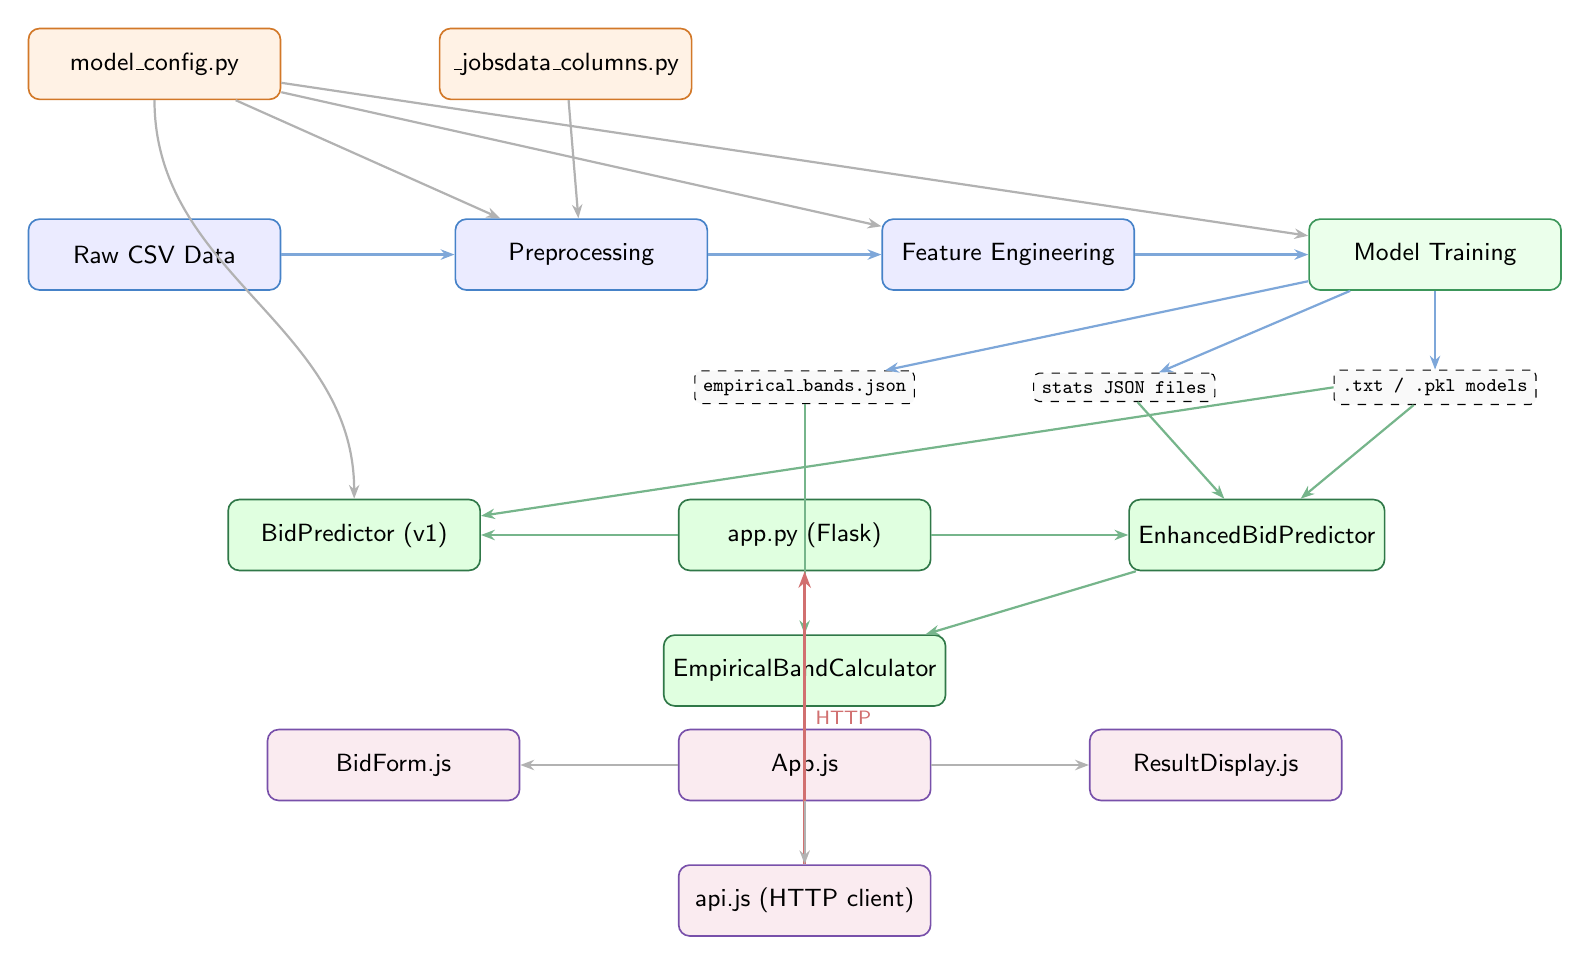
\begin{tikzpicture}[
    node distance=1.2cm and 2.5cm,
    box/.style={draw, rounded corners=4pt, minimum width=3.2cm, minimum height=0.9cm,
                font=\small\sffamily, text centered, line width=0.6pt},
    data/.style={box, fill=blue!8, draw=pipeblue},
    model/.style={box, fill=green!8, draw=apigreen},
    api/.style={box, fill=green!12, draw=apigreen!80!black},
    ui/.style={box, fill=purple!8, draw=uipurple},
    config/.style={box, fill=orange!10, draw=configorange},
    file/.style={draw, dashed, rounded corners=2pt, fill=gray!5, font=\ttfamily\scriptsize,
                 inner sep=3pt},
    arr/.style={-{Stealth[length=5pt]}, thick, color=gray!60},
    dataarr/.style={-{Stealth[length=5pt]}, thick, color=pipeblue!70},
    apiarr/.style={-{Stealth[length=5pt]}, thick, color=apigreen!70},
    httparr/.style={-{Stealth[length=6pt]}, very thick, color=gssred!70},
]

% --- Config layer ---
\node[config] (cfg) {model\_config.py};
\node[config, right=2cm of cfg] (cols) {\_jobsdata\_columns.py};

% --- Pipeline layer ---
\node[data, below=1.5cm of cfg] (raw) {Raw CSV Data};
\node[data, right=2.2cm of raw] (prep) {Preprocessing};
\node[data, right=2.2cm of prep] (feat) {Feature Engineering};
\node[model, right=2.2cm of feat] (train) {Model Training};

% --- Artifacts ---
\node[file, below=1cm of train] (models) {.txt / .pkl models};
\node[file, left=1.5cm of models] (stats) {stats JSON files};
\node[file, left=1.5cm of stats] (bands) {empirical\_bands.json};

% --- API layer ---
\node[api, below=1.2cm of bands] (apppy) {app.py (Flask)};
\node[api, right=2.5cm of apppy] (eps) {EnhancedBidPredictor};
\node[api, left=2.5cm of apppy] (ps) {BidPredictor (v1)};
\node[api, below=0.8cm of apppy] (eb) {EmpiricalBandCalculator};

% --- Frontend layer ---
\node[ui, below=2cm of apppy] (app) {App.js};
\node[ui, left=2cm of app] (form) {BidForm.js};
\node[ui, right=2cm of app] (result) {ResultDisplay.js};
\node[ui, below=0.8cm of app] (apijs) {api.js (HTTP client)};

% --- Arrows: Config → Pipeline ---
\draw[arr] (cfg) -- (prep);
\draw[arr] (cfg) -- (feat);
\draw[arr] (cfg) -- (train);
\draw[arr] (cols) -- (prep);

% --- Arrows: Pipeline flow ---
\draw[dataarr] (raw) -- (prep);
\draw[dataarr] (prep) -- (feat);
\draw[dataarr] (feat) -- (train);

% --- Arrows: Training → Artifacts ---
\draw[dataarr] (train) -- (models);
\draw[dataarr] (train) -- (stats);
\draw[dataarr] (train) -- (bands);

% --- Arrows: Artifacts → API ---
\draw[apiarr] (models) -- (eps);
\draw[apiarr] (stats) -- (eps);
\draw[apiarr] (bands) -- (eb);
\draw[apiarr] (models.west) -- (ps);

% --- Arrows: API internal ---
\draw[apiarr] (apppy) -- (eps);
\draw[apiarr] (apppy) -- (ps);
\draw[apiarr] (eps) -- (eb);

% --- Arrows: Config → API ---
\draw[arr] (cfg) to[out=-90,in=90] (ps);

% --- Arrows: Frontend → API ---
\draw[httparr] (apijs) -- node[right,font=\scriptsize\sffamily,color=gssred!70]{HTTP} (apppy);
\draw[arr] (app) -- (form);
\draw[arr] (app) -- (result);
\draw[arr] (app) -- (apijs);

\end{tikzpicture}
\end{center}

%============================================================================
\section{Codebase Inventory}
%============================================================================

\begin{longtable}{l r l l}
\toprule
\textbf{File} & \textbf{Lines} & \textbf{Layer} & \textbf{Classes / Functions} \\
\midrule
\endhead
\multicolumn{4}{l}{\textbf{\color{configorange}Configuration}} \\
\file{config/model\_config.py} & 269 & Config & 0 classes, 0 functions \\
\file{scripts/\_jobsdata\_columns.py} & 175 & Config & 0 classes, 1 list constant \\
\midrule
\multicolumn{4}{l}{\textbf{\color{pipeblue}ML Pipeline (scripts/)}} \\
\file{01\_eda.py} & 886 & EDA & 0 classes, exploratory \\
\file{02\_data\_preprocessing.py} & 613 & Prep & 1 class, 15 methods \\
\file{03\_feature\_engineering.py} & 591 & FE & 1 class, 15 methods \\
\file{04\_model\_lightgbm.py} & 764 & Model & 1 class, 12 methods \\
\file{15\_win\_probability\_baseline.py} & 525 & Model & 1 class, $\sim$10 methods \\
\file{20\_jobsdata\_eda.py} & 652 & EDA & 0 classes, exploratory \\
\file{21\_jobsdata\_preprocessing.py} & 445 & Prep & 1 class, 7+ methods \\
\file{22\_combined\_data\_preprocessing.py} & 359 & Prep & 0 classes, 5 functions \\
\file{23\_enhanced\_feature\_engineering.py} & 488 & FE & 0 classes, 4 functions \\
\file{24\_enhanced\_bidfee\_model.py} & 400 & Model & 1 class, 6 methods \\
\file{25\_enhanced\_win\_probability.py} & 473 & Model & pipeline script \\
\file{26\_enhanced\_model\_validation.py} & 222 & Eval & comparison script \\
\file{27\_generate\_api\_stats\_v2.py} & 202 & Stats & 0 classes, 2 functions \\
\file{28\_generate\_zip\_lookup.py} & 185 & Stats & 0 classes, 1 function \\
\file{28\_price\_ratio\_win\_prob.py} & 501 & Experiment & price\_ratio model \\
\file{29\_fee\_sensitive\_win\_prob.py} & 704 & Experiment & LOO v3 model \\
\file{30\_cross\_validation.py} & 247 & Eval & 0 classes, 2 functions \\
\file{33\_predict\_demo.py} & 341 & Demo & 0 classes, 1 function \\
\midrule
\multicolumn{4}{l}{\textbf{\color{apigreen}API Layer (api/)}} \\
\file{app.py} & 486 & Router & 0 classes, 12 route functions \\
\file{prediction\_service.py} & 900 & Service & 1 class, 12 methods \\
\file{enhanced\_prediction\_service.py} & 1076 & Service & 1 class, 12 methods \\
\file{empirical\_bands.py} & 312 & Utility & 1 class, 6 methods \\
\midrule
\multicolumn{4}{l}{\textbf{\color{uipurple}Frontend (frontend/src/)}} \\
\file{App.js} & 198 & Container & 1 component, 4 functions \\
\file{services/api.js} & 170 & HTTP & 0 components, 8 functions \\
\file{components/BidForm.js} & 208 & Form & 1 component \\
\file{components/ResultDisplay.js} & 543 & Display & 2 components, 5 helpers \\
\file{components/Header.js} & 20 & UI & 1 component \\
\file{components/SegmentStats.js} & 88 & UI & 1 component \\
\file{components/StateBenchmarks.js} & 112 & UI & 1 component \\
\file{components/FeeSensitivityCharts.js} & 69 & Chart & 1 component \\
\midrule
\multicolumn{4}{l}{\textbf{Tests}} \\
\file{tests/test\_validation.py} & 435 & Test & 34 test methods \\
\file{tests/test\_models.py} & 292 & Test & model-dependent tests \\
\midrule
\textbf{Total} & \textbf{$\sim$12{,}800} & & \\
\bottomrule
\end{longtable}

%============================================================================
\section{Configuration Layer}
\label{sec:config}
%============================================================================

\subsection{\file{config/model\_config.py} \conftag{269 lines}}

The single source of truth for all paths, hyperparameters, and feature exclusion lists.
Every pipeline script and both API prediction services import from this file.

\begin{longtable}{l l p{7.5cm}}
\toprule
\textbf{Constant} & \textbf{Line} & \textbf{Purpose} \\
\midrule
\endhead
\texttt{ROOT\_DIR, DATA\_DIR, ...} & 1--20 & All filesystem paths \\
\texttt{DATA\_START\_DATE} & & \texttt{"2023-01-01"} --- v1 uses 2023+ data only \\
\texttt{MIN\_TRAINING\_FEE} & & Minimum \$100 fee filter \\
\texttt{EXCLUDE\_COLUMNS} & & 13 IDs/targets/dates excluded from features \\
\texttt{JOBDATA\_FEATURES\_TO\_EXCLUDE} & & 26 JobData features that degrade performance \\
\texttt{LEAKY\_JOB\_DERIVED\_FEATURES} & & JobCount, IECount, LeaseCount, SaleCount \\
\texttt{LIGHTGBM\_CONFIG} & & Phase 1A hyperparameters: leaves=18, LR=0.02, depth=8 \\
\texttt{TRAIN\_TEST\_SPLIT} & & 60/20/20 time-based ratios \\
\texttt{PREDICTION\_CONFIG} & & Runtime clamps: \texttt{win\_prob\_min=0.05}, \texttt{win\_prob\_max=0.95} \\
\texttt{EVALUATION\_METRICS} & & Regression + classification metric lists \\
\bottomrule
\end{longtable}

\textbf{Imported by:} Every script (02--33), \file{prediction\_service.py}, \file{enhanced\_prediction\_service.py}, \file{empirical\_bands.py}.

\subsection{\file{scripts/\_jobsdata\_columns.py} \conftag{175 lines}}

Maps 143 column indices to names for the headerless \file{JobsData.csv}. Contains
\texttt{JOBSDATA\_COLUMNS} list with columns grouped into: Core Job Info (0--7),
Classification (8--14), Temporal (15--27), Geography (28--31), Property (32--52),
Office (58--61), Client (62--66), and ZipCodeMaster Demographics (67--142).

\textbf{Imported by:} \file{21\_jobsdata\_preprocessing.py}, \file{22\_combined\_data\_preprocessing.py}, \file{27\_generate\_api\_stats\_v2.py}, \file{28\_generate\_zip\_lookup.py}.

%============================================================================
\section{Data Pipeline --- Preprocessing}
\label{sec:preprocessing}
%============================================================================

\subsection{\file{scripts/02\_data\_preprocessing.py} \pipetag{613 lines}}

\cls{BidDataPreprocessor} \lineref{36} --- Transforms raw BidData CSV into a clean
dataset ready for feature engineering. Handles the entire v1 data cleaning pipeline.

\begin{longtable}{l l p{8cm}}
\toprule
\textbf{Method} & \textbf{Line} & \textbf{What It Does} \\
\midrule
\endhead
\func{\_\_init\_\_} & 39 & Sets paths, initializes \texttt{df\_raw}, \texttt{df\_clean} \\
\func{load\_data} & 61 & Reads raw CSV, converts \texttt{BidDate} to datetime \\
\func{handle\_duplicate\_bidids} & 84 & Aggregates Master/SubJob rows: max BidFee, sum counts, first for categoricals \\
\func{filter\_relevant\_bids} & 188 & Keeps only Won/Lost/Placed; drops Active/Declined/Approved \\
\func{handle\_missing\_target\_variable} & 227 & Removes rows with null BidFee \\
\func{handle\_outliers\_in\_bidfee} & 254 & Caps BidFee at 99th percentile; saves original \\
\func{handle\_missing\_targettime} & 293 & Imputes TargetTime via group median (PropertyType $\times$ BidStatus) \\
\func{handle\_missing\_categorical\_features} & 346 & Fills 15 categorical columns with ``Unknown'' \\
\func{handle\_outliers\_numerical\_features} & 388 & Caps 6 numerical columns at 99th percentile \\
\func{create\_temporal\_features} & 413 & Extracts Year/Quarter/Month/DayOfWeek + cyclical sin/cos \\
\func{create\_target\_variable\_for\_classification} & 439 & Binary target: Won=1, else=0 \\
\func{validate\_data\_quality} & 459 & Checks for nulls in critical columns \\
\func{save\_processed\_data} & 496 & Writes \file{BidData\_processed.csv} \\
\func{generate\_preprocessing\_report} & 513 & Writes JSON report with row counts \& quality stats \\
\func{run\_full\_preprocessing} & 567 & Orchestrates all steps in sequence \\
\bottomrule
\end{longtable}

\textbf{Reads:} \file{data/processed/BidData\_cleaned.csv}\\
\textbf{Writes:} \file{data/processed/BidData\_processed.csv}, \file{outputs/reports/preprocessing\_report.json}

\subsection{\file{scripts/21\_jobsdata\_preprocessing.py} \pipetag{445 lines}}

\cls{JobsDataPreprocessor} \lineref{70} --- Cleans the larger JobsData (215K rows,
2018+) for v2 training.

\begin{longtable}{l l p{8cm}}
\toprule
\textbf{Method} & \textbf{Line} & \textbf{What It Does} \\
\midrule
\endhead
\func{load\_data} & 77 & Reads raw JobsData with \texttt{JOBSDATA\_COLUMNS} headers \\
\func{filter\_closed\_recent} & 94 & Keeps Closed jobs from 2018 onward \\
\func{clean\_netfee} & 116 & Removes null/zero fees; caps at 99th percentile \\
\func{handle\_job\_types} & 149 & Deduplicates by JobId, keeps max NetFee \\
\func{clean\_categorical\_features} & 173 & Collapses rare SubType/SpecificUse ($<$50 count) to ``Other''; standardizes case \\
\func{clean\_joblength} & 230 & Parses JobLength\_Days, clamps to [1,\,365], imputes by PropertyType median \\
\func{clean\_numeric\_features} & 263 & Converts ``NULL'' strings, caps at 99th percentile, fixes YearBuilt \\
\bottomrule
\end{longtable}

\textbf{Reads:} \file{data/raw/JobsData.csv}\\
\textbf{Writes:} \file{data/processed/JobsData\_processed.csv}\\
\textbf{Imports:} \file{\_jobsdata\_columns.py} for column names

\subsection{\file{scripts/22\_combined\_data\_preprocessing.py} \pipetag{359 lines}}

Enriches BidData with JobsData features for v2 win probability training.
Module-level functions (no class).

\begin{longtable}{l l p{8cm}}
\toprule
\textbf{Function} & \textbf{Line} & \textbf{What It Does} \\
\midrule
\endhead
\func{load\_biddata} & 70 & Loads BidData\_cleaned.csv, creates Won flag \\
\func{load\_jobsdata} & 89 & Loads raw JobsData with column headers, cleans types \\
\func{enrich\_won\_bids} & 126 & LEFT JOIN on JobId: extracts SubType, GrossBuildingSF, OfficeRegion, demographics \\
\func{enrich\_lost\_bids} & 184 & Office/property-level medians: approximates JobsData values for bids that lost \\
\func{combine\_and\_finalize} & 264 & Concatenates Won + Lost, aligns columns, fills remaining NaN \\
\bottomrule
\end{longtable}

\textbf{Reads:} \file{data/processed/BidData\_cleaned.csv}, \file{data/raw/JobsData.csv}\\
\textbf{Writes:} \file{data/processed/BidData\_enriched\_v2.csv}

\textbf{Important:} Won bids get real JobsData values; lost bids get office/property
medians. This \emph{differential imputation} is a known leakage vector --- the v2 win
prob model excludes all 42 differentially-imputed features and their derivatives.

%============================================================================
\section{Data Pipeline --- Feature Engineering}
\label{sec:feature-eng}
%============================================================================

\subsection{\file{scripts/03\_feature\_engineering.py} \pipetag{591 lines}}

\cls{BidFeatureEngineer} \lineref{36} --- Creates 68+ features from processed BidData
for v1 models. All target-derived features use leave-one-out aggregation to prevent
leakage.

\begin{longtable}{l l l p{5.5cm}}
\toprule
\textbf{Method} & \textbf{Line} & \textbf{Features} & \textbf{What It Creates} \\
\midrule
\endhead
\func{create\_rolling\_features\_by\_group} & 76 & 3 & Rolling avg/std fee by segment \& office (window=10) \\
\func{create\_lag\_features\_by\_client} & 116 & 3 & lag1/lag2 BidFee, lag1 TargetTime per client \\
\func{create\_cumulative\_client\_features} & 147 & 3 & Expanding bids/wins/winrate per client \\
\func{create\_aggregation\_features} & 179 & 15 & LOO avg\_fee, std\_fee, win\_rate for 5 groups \\
\func{create\_competitiveness\_features} & 239 & 5 & bid\_vs\_segment\_ratio, fee\_diff, fee\_percentile \\
\func{create\_temporal\_behavioral\_features} & 285 & 9 & days\_since\_last\_bid, bid\_count\_30d, calendar features \\
\func{create\_market\_dynamics\_features} & 336 & 4 & bid\_density, combo\_freq, specialization, workload \\
\func{create\_risk\_volatility\_features} & 378 & 4 & segment CV, client consistency, targettime ratio \\
\func{create\_interaction\_features} & 417 & 6 & Cross-feature products (fee $\times$ time, etc.) \\
\func{create\_categorical\_encodings} & 461 & 2 & Frequency encoding for segment \& property type \\
\bottomrule
\end{longtable}

\textbf{Total features created:} 54 engineered + 14 temporal (from script 02) = 68\\
\textbf{Reads:} \file{data/processed/BidData\_processed.csv}\\
\textbf{Writes:} \file{data/features/bid\_features.csv}

\subsection{\file{scripts/23\_enhanced\_feature\_engineering.py} \pipetag{488 lines}}

Creates v2 features for \emph{both} Phase 1A (JobsData \arrow\ NetFee) and Phase 1B
(enriched BidData \arrow\ Win). Uses shared \func{build\_common\_features} to ensure
consistency.

\begin{longtable}{l l p{8cm}}
\toprule
\textbf{Function} & \textbf{Line} & \textbf{What It Does} \\
\midrule
\endhead
\func{leave\_one\_out\_mean} & 58 & LOO aggregation: excludes current row from group mean \\
\func{frequency\_encode} & 65 & Maps category \arrow\ raw count (min\_count=10) \\
\func{build\_common\_features} & 71 & Shared engine: LOO aggregates (segment, state, property type), rolling features, frequency encoding, JobLength features (log, bucket, $\times$ segment), building area (log, fee/sqft), interaction terms, temporal features, zip demographics \\
\func{engineer\_phase1a\_features} & 265 & Calls \func{build\_common\_features} on JobsData with NetFee target \\
\bottomrule
\end{longtable}

\textbf{Key v2 additions:} SubType features (\func{subtype\_avg\_fee}, \func{subtype\_frequency}),
OfficeRegion features (\func{office\_region\_avg\_fee}), CompanyLocation frequency,
JobLength derivatives, building area features, zip demographics (15 columns),
\func{income\_x\_segment\_fee}, \func{pop\_density\_log}.

\textbf{Reads:} \file{data/processed/JobsData\_processed.csv}, \file{data/processed/BidData\_enriched\_v2.csv}\\
\textbf{Writes:} \file{data/features/JobsData\_features\_v2.csv}, \file{data/features/BidData\_features\_v2.csv}

%============================================================================
\section{Data Pipeline --- Model Training}
\label{sec:training}
%============================================================================

\subsection{\file{scripts/04\_model\_lightgbm.py} \pipetag{764 lines} --- Phase 1A v1}

\cls{LightGBMBidFeePredictor} \lineref{57} --- Trains the v1 bid fee regression model.

\begin{longtable}{l l p{8cm}}
\toprule
\textbf{Method} & \textbf{Line} & \textbf{What It Does} \\
\midrule
\endhead
\func{load\_data} & 96 & Loads features CSV; filters to 2023+ \\
\func{select\_top\_features} & 178 & Reduces to top 68 via \file{selected\_features\_top68.csv} \\
\func{prepare\_features} & 226 & Excludes ID/target columns; selects numeric only \\
\func{time\_based\_split} & 286 & Chronological 60/20/20 split \\
\func{train\_model} & 350 & Applies \texttt{log1p} transform; trains LightGBM with early stopping (1500 rounds) \\
\func{evaluate\_model} & 428 & Inverts \texttt{expm1}; computes RMSE (\$531), MAPE (15.7\%), R\textsuperscript{2} (0.94) \\
\func{feature\_importance\_analysis} & 537 & Top 30 features by gain; saves CSV + plot \\
\func{shap\_analysis} & 586 & SHAP summary on test sample \\
\func{save\_model} & 631 & Writes \texttt{.txt} model + metadata JSON + predictions CSV \\
\func{run\_full\_pipeline} & 693 & Orchestrates all steps \\
\bottomrule
\end{longtable}

\textbf{Reads:} \file{data/features/bid\_features.csv}, \file{outputs/reports/selected\_features\_top68.csv}\\
\textbf{Writes:} \file{outputs/models/lightgbm\_bidfee\_model.txt}, \file{outputs/models/lightgbm\_metadata.json}

\subsection{\file{scripts/24\_enhanced\_bidfee\_model.py} \pipetag{400 lines} --- Phase 1A v2}

\cls{EnhancedBidFeePredictor} \lineref{108} --- Trains v2 bid fee model on JobsData (215K rows).

\begin{longtable}{l l p{8cm}}
\toprule
\textbf{Method} & \textbf{Line} & \textbf{What It Does} \\
\midrule
\endhead
\func{load\_data} & 117 & Loads JobsData features; filters 2018+ and fee $\geq$ MIN\_TRAINING\_FEE \\
\func{prepare\_features} & 144 & Excludes IDs, targets, categoricals, leaky features \\
\func{time\_based\_split} & 162 & Chronological 60/20/20 \\
\func{train} & 187 & \texttt{log1p} transform; 3000 rounds, early stop=150 \\
\func{evaluate} & 218 & MAPE 7.3\%, R\textsuperscript{2} 0.924, overfit 2.09$\times$ \\
\func{feature\_importance} & 269 & Saves importance CSV + plot \\
\bottomrule
\end{longtable}

\textbf{v2 hyperparameters:} leaves=18, LR=0.02, depth=6, \texttt{reg\_alpha=20.0}, \texttt{reg\_lambda=20.0} (heavy regularization).\\
\textbf{Writes:} \file{outputs/models/lightgbm\_bidfee\_v2\_model.txt}, \file{outputs/models/lightgbm\_bidfee\_v2\_metadata.json}

\subsection{\file{scripts/15\_win\_probability\_baseline.py} \pipetag{525 lines} --- Phase 1B v1}

Trains v1 win probability classifier. Uses 72 features including BidFee as a direct
input (the model learns fee-sensitivity from data). Excludes
\texttt{LEAKY\_JOB\_DERIVED\_FEATURES} and win-rate features.

\textbf{Key metrics:} AUC 0.870, accuracy 79.0\%, overfit 1.09$\times$.\\
\textbf{Writes:} \file{outputs/models/lightgbm\_win\_probability.txt}, metadata JSON

\subsection{\file{scripts/25\_enhanced\_win\_probability.py} \pipetag{473 lines} --- Phase 1B v2}

Trains v2 win probability on enriched BidData (2018+). Excludes all 42
differentially-imputed Jobs\_* features plus their derivatives (fee\_per\_sqft,
building\_sf\_log, etc.) to prevent leakage.

\textbf{Key metrics:} AUC 0.948, accuracy 86.7\%, overfit 1.04$\times$, 44 features.

\textbf{Known issue:} Model is \textbf{saturated at inference} --- raw output is
0.97--0.98 for all inputs. BidFee is not in the top 10 features.
\texttt{subtype\_frequency} (31\%) and \texttt{office\_region\_avg\_fee} (25\%) dominate.
The API falls back to a heuristic sigmoid when this is detected.

%============================================================================
\section{Data Pipeline --- Stats Generation}
\label{sec:stats-gen}
%============================================================================

\subsection{\file{scripts/27\_generate\_api\_stats\_v2.py} \pipetag{202 lines}}

Pre-computes all runtime lookup tables consumed by the API at startup.

\begin{longtable}{l l p{8cm}}
\toprule
\textbf{Function} & \textbf{Line} & \textbf{What It Produces} \\
\midrule
\endhead
\func{generate\_phase1a\_stats} & 30 & Global stats, dropdown options, per-segment/state/property/subtype/office averages, rolling proxies, state coordinates, SubType-by-PropertyType cascading map \\
\func{generate\_feature\_defaults} & 148 & Per-feature global median/mean + segment-specific medians \\
\bottomrule
\end{longtable}

\textbf{Writes:} \file{outputs/reports/api\_precomputed\_stats\_v2.json}, \file{outputs/reports/feature\_defaults\_v2.json}

\subsection{\file{scripts/28\_generate\_zip\_lookup.py} \pipetag{185 lines}}

\func{generate\_zip\_lookup} \lineref{58} --- Builds a static dictionary mapping
20,040 zip codes to demographics (15 features), state, lat/lon, distance, and sample
count. Only includes zips with $\geq$5 demographic values.

\textbf{Writes:} \file{outputs/reports/zip\_demographics\_lookup.json}

%============================================================================
\section{API Layer --- Flask Backend}
\label{sec:api}
%============================================================================

\subsection{\file{api/app.py} \apitag{486 lines} --- HTTP Router}

Flask application with CORS. Lazy-loads v1 and v2 predictors on first request.

\begin{longtable}{l l l p{5cm}}
\toprule
\textbf{Endpoint} & \textbf{Method} & \textbf{Line} & \textbf{Purpose} \\
\midrule
\endhead
\texttt{/api/ping} & GET & 38 & Liveness check \\
\texttt{/api/debug} & GET & 68 & File status, init errors \\
\texttt{/api/health} & GET & 139 & Health check (Render uptime) \\
\texttt{/api/options} & GET & 152 & v1 dropdown data \\
\texttt{/api/predict} & POST & 168 & v1 prediction \\
\texttt{/api/segment/<name>} & GET & 239 & v1 segment stats \\
\texttt{/api/batch-predict} & POST & 256 & v1 batch prediction \\
\texttt{/api/v2/options} & GET & 314 & v2 dropdown data (incl.\ subtypes, regions) \\
\texttt{/api/v2/predict} & POST & 329 & \textbf{v2 prediction (active)} \\
\texttt{/api/v2/zip/<code>} & GET & 380 & Zip lookup + state resolution \\
\texttt{/api/v2/segment/<name>} & GET & 414 & v2 segment stats \\
\bottomrule
\end{longtable}

\textbf{Imports:} \file{prediction\_service.get\_predictor}, \file{enhanced\_prediction\_service.EnhancedBidPredictor}

\subsection{\file{api/prediction\_service.py} \apitag{900 lines} --- v1 Prediction Engine}

\cls{BidPredictor} \lineref{49} --- Full v1 inference pipeline.

\begin{longtable}{l l p{7.5cm}}
\toprule
\textbf{Method} & \textbf{Line} & \textbf{What It Does} \\
\midrule
\endhead
\func{\_\_init\_\_} & 56 & Loads v1 models, stats, defaults, bands, zip data \\
\func{\_load\_model} & 76 & Reads \file{lightgbm\_bidfee\_model.txt} \\
\func{\_load\_win\_probability\_model} & 88 & Reads \file{lightgbm\_win\_probability.txt} + metadata \\
\func{\_compute\_feature\_statistics} & 109 & Loads \file{api\_precomputed\_stats.json}; computes global/segment/state/property/office averages \\
\func{\_load\_empirical\_bands} & 223 & Instantiates \cls{EmpiricalBandCalculator}, loads \file{empirical\_bands.json} \\
\func{\_load\_feature\_defaults} & 236 & Loads \file{feature\_defaults.json}, \file{state\_coordinates.json}, \file{rolling\_stats.json} \\
\func{\_generate\_features} & 271 & \textbf{Maps 6 raw inputs \arrow\ 68 features.} 15 feature categories: raw inputs, segment/state/property/office aggregates, rolling, client history, competitiveness, temporal (sin/cos), market dynamics, risk, interactions, demographics \\
\func{predict} & 506 & \textbf{Main entry.} generate features \arrow\ predict fee (\texttt{expm1}) \arrow\ floor enforcement \arrow\ confidence interval \arrow\ inject fee as BidFee \arrow\ predict win prob \arrow\ calculate EV \arrow\ build recommendation \\
\func{predict\_win\_probability} & 729 & Builds win prob feature vector; predicts with v1 classifier; clamps [0.05, 0.95] \\
\func{\_fallback\_win\_probability} & 798 & Sigmoid heuristic: $P = 1/(1+e^{5(\text{ratio}-1)})$ scaled to [0.20, 0.75] \\
\func{get\_dropdown\_options} & 711 & Returns segments, property types, states, offices \\
\func{get\_segment\_stats} & 720 & Returns per-segment avg/std/winrate/count \\
\bottomrule
\end{longtable}

\textbf{Runtime files loaded:} \file{lightgbm\_bidfee\_model.txt}, \file{lightgbm\_win\_probability.txt}, \file{api\_precomputed\_stats.json}, \file{feature\_defaults.json}, \file{state\_coordinates.json}, \file{rolling\_stats.json}, \file{empirical\_bands.json}

\subsection{\file{api/enhanced\_prediction\_service.py} \apitag{1076 lines} --- v2 Prediction Engine}

\cls{EnhancedBidPredictor} \lineref{158} --- The production-active v2 engine with fee
sensitivity curves, EV optimization, saturation detection, and heuristic fallback.

\subsubsection{Module-Level Constants \& Functions}

\begin{longtable}{l l p{7.5cm}}
\toprule
\textbf{Name} & \textbf{Line} & \textbf{Description} \\
\midrule
\endhead
\texttt{LOCATION\_TO\_REGION} & 47 & Dict mapping 30+ office location names \arrow\ 6 regions \\
\texttt{SATURATION\_THRESHOLD} & 134 & 0.93 --- raw model output above this triggers heuristic \\
\texttt{CURVE\_FLAT\_THRESHOLD\_PP} & 135 & 5.0 --- curve spread below this (pp) is replaced with heuristic \\
\func{\_heuristic\_win\_prob(fee, blended)} & 138 & Logistic fallback: $P = 0.22 + \frac{0.58}{1 + e^{3.5(r - 1.0)}}$ where $r = \text{fee}/\text{blended}$ \\
\bottomrule
\end{longtable}

\subsubsection{Class Methods}

\begin{longtable}{l l p{7.5cm}}
\toprule
\textbf{Method} & \textbf{Line} & \textbf{What It Does} \\
\midrule
\endhead
\func{\_\_init\_\_} & 161 & Loads v2 models, stats, defaults, zip lookup, bands; runs startup canary \\
\func{\_load\_models} & 179 & Reads v2 \texttt{.txt} models + isotonic calibrator pickle \\
\func{\_load\_stats} & 212 & Reads \file{api\_precomputed\_stats\_v2.json} \\
\func{\_load\_zip\_lookup} & 236 & Reads \file{zip\_demographics\_lookup.json} (20K zips) \\
\func{\_run\_startup\_canary} & 246 & Tests v2 win prob at 3 fees (\$500/\$3K/\$10K); logs WARNING if saturated \\
\func{\_generate\_features} & 296 & \textbf{Maps raw inputs + zip \arrow\ 44+ features.} Segment, state, property, subtype, office region, company location, rolling, interactions, temporal (sin/cos), geographic (lat/lon from zip), JobLength (log, bucket), building area, 15 zip demographics, distance \\
\func{predict} & 476 & \textbf{Main entry.} Derives office\_region \arrow\ parse date \arrow\ validate zip \arrow\ generate features \arrow\ predict fee (\texttt{expm1}) \arrow\ benchmark floor \arrow\ rare-combo blending \arrow\ confidence interval \arrow\ blended benchmark \arrow\ inject fee \arrow\ predict win prob (with saturation detection) \arrow\ EV \arrow\ fee sensitivity curve (20 points, 0.4$\times$ to 2.0$\times$) \arrow\ EV optimization \arrow\ solid win ceiling (30\% threshold) \arrow\ build recommendation \arrow\ warnings \\
\func{\_predict\_win\_probability} & 730 & Builds vector; predicts raw; \textbf{if raw $\geq$ 0.93: returns heuristic}; else applies isotonic calibration; clamps [0.05, 0.95] \\
\func{get\_fee\_sensitivity\_curve} & 835 & Sweeps 20 fee points; calls \func{\_predict\_win\_probability} for each; \textbf{if flat ($<$5pp spread): replaces entire curve with heuristic} \\
\func{\_build\_recommendation} & 898 & 5 fee tiers $\times$ 3 win tiers = 15 headline combinations; adds market context, strategy tips, low-confidence notes, frontend signal \\
\func{get\_dropdown\_options} & 1058 & v2 options including subtypes\_by\_property\_type cascading map \\
\bottomrule
\end{longtable}

\textbf{Runtime files loaded:} \file{lightgbm\_bidfee\_v2\_model.txt}, \file{lightgbm\_win\_probability\_v2.txt}, \file{win\_probability\_v2\_calibrator.pkl}, \file{api\_precomputed\_stats\_v2.json}, \file{feature\_defaults\_v2.json}, \file{zip\_demographics\_lookup.json}, \file{empirical\_bands.json}

\subsection{\file{api/empirical\_bands.py} \apitag{312 lines} --- Confidence Intervals}

\cls{EmpiricalBandCalculator} \lineref{27} --- Computes quantile-based confidence
intervals from historical prediction residuals, stratified by fee bucket, segment, and state.

\begin{longtable}{l l p{8cm}}
\toprule
\textbf{Method} & \textbf{Line} & \textbf{What It Does} \\
\midrule
\endhead
\func{compute\_bands\_from\_predictions} & 45 & Computes residual quantiles: global, by fee bucket (4 buckets), by segment ($\geq$30 samples), by state ($\geq$50 samples) \\
\func{\_compute\_quantiles} & 95 & Returns p5, p10, p25, p50, p75, p90, p95, std, n for a residual array \\
\func{get\_confidence\_interval} & 109 & \textbf{Fallback hierarchy:} segment \arrow\ state \arrow\ fee bucket \arrow\ global. Selects quantile pair by confidence level (80\% \arrow\ p10/p90). Enforces $\geq$\$500 floor and $\geq$\$100 width \\
\func{save\_bands / load\_bands} & 201/219 & JSON serialization to/from \file{empirical\_bands.json} \\
\bottomrule
\end{longtable}

\textbf{Fee buckets:} low (0--2K), medium (2K--4K), high (4K--6K), very\_high (6K+).\\
\textbf{Imported by:} \file{prediction\_service.py}, \file{enhanced\_prediction\_service.py}

%============================================================================
\section{v2 Prediction Request --- Complete Data Flow}
\label{sec:dataflow}
%============================================================================

This traces a single \texttt{POST /api/v2/predict} request from HTTP arrival to JSON
response.

\begin{enumerate}[leftmargin=2em]
    \item \textbf{\file{app.py}:329} --- Flask receives POST. Extracts 7 fields from JSON body.

    \item \textbf{\file{app.py}:364} --- Calls \func{enhanced\_predictor.predict(...)}

    \item \textbf{\file{enhanced\_prediction\_service.py}:493} --- Derives \texttt{office\_region} from \texttt{LOCATION\_TO\_REGION} dict.

    \item \textbf{:496} --- Parses \texttt{open\_date} string to datetime for temporal features.

    \item \textbf{:508} --- Validates \texttt{zip\_code} against \texttt{self.zip\_lookup}; detects state mismatch.

    \item \textbf{:518} --- Calls \func{\_generate\_features()} \arrow\ builds 44+ feature dict from raw inputs + precomputed stats + zip demographics.

    \item \textbf{:534} --- Orders features to match \texttt{self.model\_features} (training metadata order). Missing features filled from \texttt{self.feature\_defaults}.

    \item \textbf{:546} --- Phase 1A prediction: \texttt{model.predict(X)[0]} \arrow\ \texttt{expm1()} \arrow\ dollar amount.

    \item \textbf{:551} --- Benchmark-aware floor: $\max(\$500,\; 30\% \times \text{segment\_avg})$.

    \item \textbf{:558} --- Rare-combo blending: if sample count $<$ 100, blends prediction toward segment average.

    \item \textbf{:567} --- \cls{EmpiricalBandCalculator}.\func{get\_confidence\_interval()} \arrow\ 80\% CI with segment \arrow\ state \arrow\ bucket \arrow\ global fallback.

    \item \textbf{:597} --- Computes blended benchmark: $0.4 \times \text{seg} + 0.3 \times \text{state} + 0.3 \times \text{prop}$.

    \item \textbf{:604} --- Injects predicted fee as \texttt{BidFee} into features dict. Calls \func{\_predict\_win\_probability()}.

    \item \textbf{:771} --- Inside \func{\_predict\_win\_probability}: raw model output. If $\geq 0.93$ (saturated), returns \func{\_heuristic\_win\_prob()} instead.

    \item \textbf{:610} --- $\text{EV} = P(\text{Win}) \times \text{predicted\_fee}$.

    \item \textbf{:613} --- \func{get\_fee\_sensitivity\_curve()} sweeps 20 points from $0.4\times$ to $2.0\times$ predicted fee. Each point calls \func{\_predict\_win\_probability}. If curve is flat ($<$5pp), replaces with heuristic.

    \item \textbf{:624} --- EV optimization: finds fee point on curve that maximizes $P(\text{Win}) \times \text{fee}$.

    \item \textbf{:630} --- Solid win ceiling: highest fee with $\geq 30\%$ win probability.

    \item \textbf{:634} --- If EV-optimal fee $>$ ceiling, caps at ceiling; sets \texttt{ev\_capped\_at\_ceiling = true}.

    \item \textbf{:658} --- \func{\_build\_recommendation()} generates plain-language headline, detail, strategy tip, and signal.

    \item \textbf{:690} --- Returns complete JSON response with 15+ fields.
\end{enumerate}

%============================================================================
\section{Frontend Layer --- React}
\label{sec:frontend}
%============================================================================

\subsection{\file{frontend/src/App.js} \uitag{198 lines} --- State Container}

Root component. All state lifted here; children are presentational.

\begin{longtable}{l l p{7.5cm}}
\toprule
\textbf{State Variable} & \textbf{Line} & \textbf{Purpose} \\
\midrule
\endhead
\texttt{options} & 9 & Dropdown data from \texttt{GET /v2/options} \\
\texttt{loading} & 18 & Initial options fetch in flight \\
\texttt{predicting} & 19 & Prediction API call in flight \\
\texttt{prediction} & 20 & Full API response object \\
\texttt{error} & 21 & Error message string \\
\texttt{formData} & 24 & User input: segment, property\_type, state, turnaround\_days, zip\_code, sub\_property\_type, office\_location, open\_date \\
\texttt{zipStatus} & 34 & Zip lookup result: \{found, state, loading\} \\
\bottomrule
\end{longtable}

\begin{longtable}{l l p{7.5cm}}
\toprule
\textbf{Function} & \textbf{Line} & \textbf{What It Does} \\
\midrule
\endhead
\func{loadOptions} & 38 & Calls \func{fetchV2Options()}, sets dropdown defaults \\
\func{handleInputChange} & 65 & Updates formData; resets subtype on property\_type change; triggers zip lookup at 5 digits \\
\func{handleSubmit} & 96 & Builds payload (splits turnaround\_days into target\_time + delivery\_days); calls \func{predictV2BidFee()} \\
\func{handleReset} & 127 & Clears prediction and error \\
\bottomrule
\end{longtable}

\textbf{API calls:} \func{fetchV2Options} (mount), \func{lookupZip} (on zip input), \func{predictV2BidFee} (on submit).

\subsection{\file{frontend/src/services/api.js} \uitag{170 lines} --- HTTP Client}

All backend communication via native Fetch API.

\begin{longtable}{l l l l}
\toprule
\textbf{Function} & \textbf{Line} & \textbf{Method} & \textbf{Endpoint} \\
\midrule
\endhead
\func{fetchOptions} & 11 & GET & \texttt{/api/options} \\
\func{predictBidFee} & 30 & POST & \texttt{/api/predict} \\
\func{fetchSegmentStats} & 55 & GET & \texttt{/api/segment/\{name\}} \\
\func{batchPredict} & 74 & POST & \texttt{/api/batch-predict} \\
\func{fetchV2Options} & 99 & GET & \texttt{/api/v2/options} \\
\func{predictV2BidFee} & 118 & POST & \texttt{/api/v2/predict} \\
\func{lookupZip} & 143 & GET & \texttt{/api/v2/zip/\{code\}} \\
\func{checkHealth} & 162 & GET & \texttt{/api/health} \\
\bottomrule
\end{longtable}

\texttt{API\_BASE\_URL} \lineref{6}: \texttt{process.env.REACT\_APP\_API\_URL || '/api'}.
Production uses Vercel env var pointing to Render backend.

\subsection{\file{frontend/src/components/BidForm.js} \uitag{208 lines}}

Pure presentational form. Receives \texttt{formData}, \texttt{options}, \texttt{onChange},
\texttt{onSubmit}, \texttt{loading}, \texttt{zipStatus} as props. Contains 8 input
fields (segment, property\_type, sub\_property\_type, zip\_code, state, turnaround\_days,
open\_date, office\_location) plus turnaround preset buttons (14/21/30/45/60 days).

\textbf{No state, no API calls.} All logic delegated to parent \file{App.js}.

\subsection{\file{frontend/src/components/ResultDisplay.js} \uitag{543 lines}}

The most complex frontend component. Contains helper functions, an inner
\cls{FeeChart} component, and the main \cls{ResultDisplay} component.

\subsubsection{Helper Functions (lines 4--130)}

\begin{longtable}{l l p{7cm}}
\toprule
\textbf{Function} & \textbf{Line} & \textbf{What It Does} \\
\midrule
\endhead
\func{fmt(n)} & 6 & Formats number with locale separators (3245 \arrow\ ``3,245'') \\
\func{interpolateWinProb(fee, curve)} & 10 & Linear interpolation on fee curve to find win prob at any fee \\
\func{winLabel(pct)} & 24 & Maps \% to label: ``Strong'' / ``Moderate'' / ``Low'' \\
\func{winColor(pct)} & 31 & Maps \% to hex: green ($\geq$55\%) / amber ($\geq$35\%) / red ($<$35\%) \\
\func{buildContextMessage(\ldots)} & 39 & Client-side contextual messaging engine. 6 cases: EV-capped, flat curve, low win prob, low confidence, strong odds, moderate default. Returns \{headline, body, tip, signal\} \\
\bottomrule
\end{longtable}

\subsubsection{\cls{FeeChart} Component (lines 134--244)}

SVG-based interactive fee vs.\ win probability chart.

\textbf{State:} \texttt{chartFee} (slider position).
\textbf{Props:} \texttt{curvePoints}, \texttt{recFee}, \texttt{maxFee}, \texttt{floorFee}, \texttt{evCapped}.
\textbf{Renders:} Y-axis gridlines, fee curve polyline, 30\% viability threshold (red
dashed), floor/ceiling vertical markers, draggable slider, live stats (fee, win\%,
EV).

\subsubsection{Main \cls{ResultDisplay} Component (lines 248--541)}

\textbf{Key computed values (lines 248--311):}
\begin{lstlisting}
floorFee = confidence_interval.low
recFee   = ev_optimal_fee || predicted_fee
maxFee   = solid_win_ceiling || confidence_interval.high
evCapped = ev_capped_at_ceiling || false
winProbPct = interpolateWinProb(recFee, curvePoints)
evAtRec  = (winProbPct / 100) * recFee
vsMarket = ((recFee - segment_benchmark) / segment_benchmark * 100)
isFlatCurve = (max_prob - min_prob) < 8
\end{lstlisting}

\textbf{Render sections:}
\begin{enumerate}[leftmargin=2em]
    \item Warnings (317--322): first entry from \texttt{prediction.warnings[]}
    \item Bid Range panel (325--404): floor / optimal / ceiling with scale bar
    \item Win probability bar (407--420): colored bar + EV display
    \item Flat curve note (425--434): shown if price has little effect
    \item Contextual insight card (437--445): from \func{buildContextMessage}
    \item Fee chart (448--465): expandable \cls{FeeChart}
    \item Market context strip (468--485): segment, state, zip, vs.\ segment \%
    \item Rush callout (488--498): if turnaround $\leq$ 21 days
    \item Details panel (501--537): segment/state benchmarks, subtype/region effects
\end{enumerate}

\subsection{Other Components}

\begin{longtable}{l l l p{5.5cm}}
\toprule
\textbf{File} & \textbf{Lines} & \textbf{Component} & \textbf{Purpose} \\
\midrule
\endhead
\file{Header.js} & 20 & \cls{Header} & Static brand header \\
\file{SegmentStats.js} & 88 & \cls{SegmentStats} & Dropdown + stats grid; calls \func{fetchSegmentStats} API \\
\file{StateBenchmarks.js} & 112 & \cls{StateBenchmarks} & State comparison bars (hardcoded \texttt{STATE\_DATA}) \\
\file{FeeSensitivityCharts.js} & 69 & \cls{FeeSensitivityCharts} & Recharts LineChart for fee curve (alternative to SVG FeeChart) \\
\bottomrule
\end{longtable}

%============================================================================
\section{Cross-Module Import Map}
\label{sec:imports}
%============================================================================

\subsection{Python Backend Imports}

\begin{center}
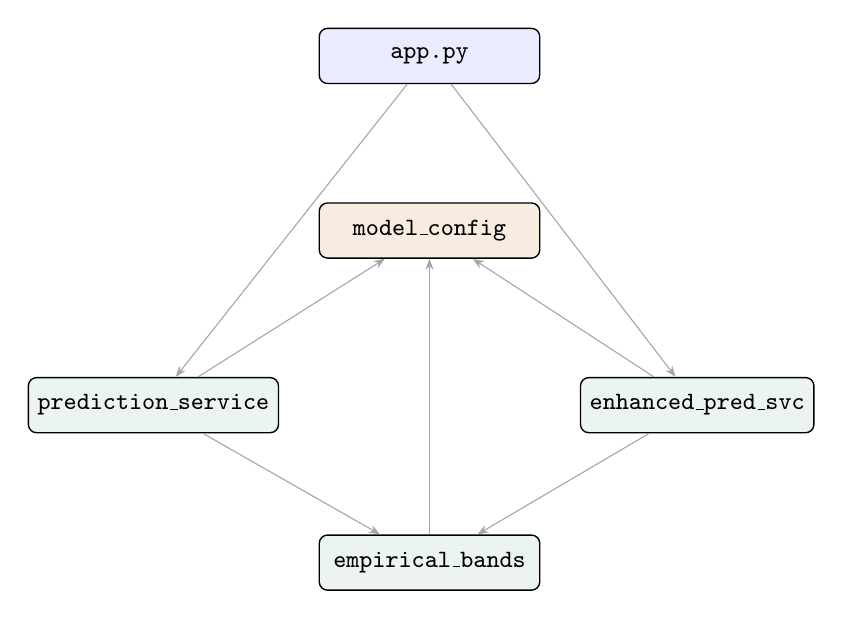
\begin{tikzpicture}[
    node distance=1cm and 2.5cm,
    mod/.style={draw, rounded corners=3pt, minimum width=2.8cm, minimum height=0.7cm,
                font=\small\ttfamily, text centered, line width=0.5pt},
    arr/.style={-{Stealth[length=4pt]}, color=gray!70},
]
\node[mod, fill=configorange!15] (cfg) {model\_config};
\node[mod, fill=apigreen!10, below left=1.5cm and 0.5cm of cfg] (ps) {prediction\_service};
\node[mod, fill=apigreen!10, below right=1.5cm and 0.5cm of cfg] (eps) {enhanced\_pred\_svc};
\node[mod, fill=apigreen!10, below=3.5cm of cfg] (eb) {empirical\_bands};
\node[mod, fill=blue!8, above=1.5cm of cfg] (app) {app.py};

\draw[arr] (app) -- (ps);
\draw[arr] (app) -- (eps);
\draw[arr] (ps) -- (cfg);
\draw[arr] (eps) -- (cfg);
\draw[arr] (eb) -- (cfg);
\draw[arr] (ps) -- (eb);
\draw[arr] (eps) -- (eb);
\end{tikzpicture}
\end{center}

\subsection{Frontend Component Tree}

\begin{center}
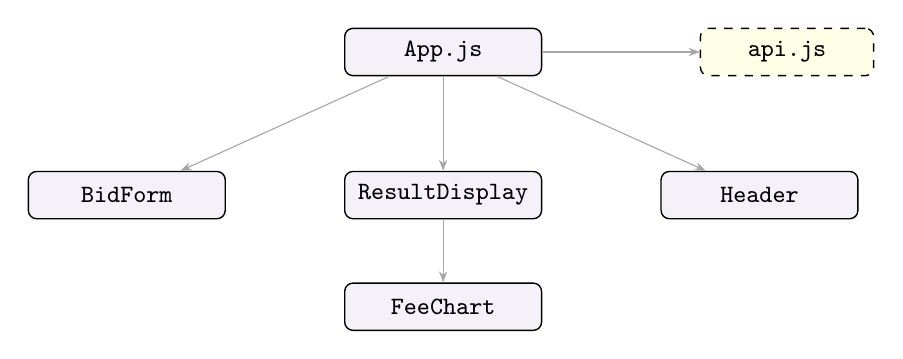
\begin{tikzpicture}[
    node distance=0.8cm and 1.5cm,
    comp/.style={draw, rounded corners=3pt, minimum width=2.5cm, minimum height=0.6cm,
                 font=\small\ttfamily, text centered, fill=uipurple!8, line width=0.5pt},
    svc/.style={draw, dashed, rounded corners=3pt, minimum width=2.2cm, minimum height=0.6cm,
                font=\small\ttfamily, text centered, fill=yellow!10, line width=0.5pt},
    arr/.style={-{Stealth[length=4pt]}, color=gray!70},
]
\node[comp] (app) {App.js};
\node[comp, below left=1.2cm and 1.5cm of app] (form) {BidForm};
\node[comp, below=1.2cm of app] (result) {ResultDisplay};
\node[comp, below right=1.2cm and 1.5cm of app] (header) {Header};
\node[comp, below=0.8cm of result] (chart) {FeeChart};
\node[svc, right=2cm of app] (api) {api.js};

\draw[arr] (app) -- (form);
\draw[arr] (app) -- (result);
\draw[arr] (app) -- (header);
\draw[arr] (result) -- (chart);
\draw[arr] (app) -- (api);
\end{tikzpicture}
\end{center}

%============================================================================
\section{File Dependency Graph --- What Reads What}
\label{sec:filedeps}
%============================================================================

Every runtime and training-time file dependency in the system:

\begin{longtable}{p{5cm} l p{6cm}}
\toprule
\textbf{Consumer} & \textbf{Direction} & \textbf{Producer} \\
\midrule
\endhead
\multicolumn{3}{l}{\textbf{Training Pipeline}} \\
\file{02\_data\_preprocessing} & reads & \file{data/processed/BidData\_cleaned.csv} \\
\file{02\_data\_preprocessing} & writes & \file{data/processed/BidData\_processed.csv} \\
\file{03\_feature\_engineering} & reads & \file{BidData\_processed.csv} \\
\file{03\_feature\_engineering} & writes & \file{data/features/bid\_features.csv} \\
\file{04\_model\_lightgbm} & reads & \file{bid\_features.csv} \\
\file{04\_model\_lightgbm} & writes & \file{lightgbm\_bidfee\_model.txt} \\
\file{15\_win\_prob\_baseline} & reads & \file{bid\_features.csv} \\
\file{15\_win\_prob\_baseline} & writes & \file{lightgbm\_win\_probability.txt} \\
\file{21\_jobsdata\_preproc} & reads & \file{data/raw/JobsData.csv} \\
\file{21\_jobsdata\_preproc} & writes & \file{data/processed/JobsData\_processed.csv} \\
\file{22\_combined\_preproc} & reads & \file{BidData\_cleaned.csv} + \file{JobsData.csv} \\
\file{22\_combined\_preproc} & writes & \file{BidData\_enriched\_v2.csv} \\
\file{23\_enhanced\_fe} & reads & \file{JobsData\_processed.csv} + \file{BidData\_enriched\_v2.csv} \\
\file{23\_enhanced\_fe} & writes & \file{JobsData\_features\_v2.csv} + \file{BidData\_features\_v2.csv} \\
\file{24\_enhanced\_bidfee} & reads & \file{JobsData\_features\_v2.csv} \\
\file{24\_enhanced\_bidfee} & writes & \file{lightgbm\_bidfee\_v2\_model.txt} \\
\file{25\_enhanced\_winprob} & reads & \file{BidData\_features\_v2.csv} \\
\file{25\_enhanced\_winprob} & writes & \file{lightgbm\_win\_probability\_v2.txt} + calibrator pkl \\
\file{27\_api\_stats\_v2} & reads & \file{JobsData\_features\_v2.csv} + model metadata \\
\file{27\_api\_stats\_v2} & writes & \file{api\_precomputed\_stats\_v2.json} + \file{feature\_defaults\_v2.json} \\
\file{28\_zip\_lookup} & reads & \file{data/raw/JobsData.csv} \\
\file{28\_zip\_lookup} & writes & \file{zip\_demographics\_lookup.json} \\
\midrule
\multicolumn{3}{l}{\textbf{API Runtime}} \\
\file{BidPredictor.\_\_init\_\_} & loads & \file{lightgbm\_bidfee\_model.txt} \\
\file{BidPredictor.\_\_init\_\_} & loads & \file{lightgbm\_win\_probability.txt} + metadata \\
\file{BidPredictor.\_\_init\_\_} & loads & \file{api\_precomputed\_stats.json} \\
\file{BidPredictor.\_\_init\_\_} & loads & \file{feature\_defaults.json} + \file{state\_coordinates.json} + \file{rolling\_stats.json} \\
\file{EnhancedBidPredictor.\_\_init\_\_} & loads & \file{lightgbm\_bidfee\_v2\_model.txt} \\
\file{EnhancedBidPredictor.\_\_init\_\_} & loads & \file{lightgbm\_win\_probability\_v2.txt} + calibrator \\
\file{EnhancedBidPredictor.\_\_init\_\_} & loads & \file{api\_precomputed\_stats\_v2.json} \\
\file{EnhancedBidPredictor.\_\_init\_\_} & loads & \file{feature\_defaults\_v2.json} \\
\file{EnhancedBidPredictor.\_\_init\_\_} & loads & \file{zip\_demographics\_lookup.json} \\
\file{EmpiricalBandCalculator} & loads & \file{empirical\_bands.json} \\
\midrule
\multicolumn{3}{l}{\textbf{Frontend \arrow\ API (HTTP)}} \\
\file{App.js} & GET & \texttt{/api/v2/options} \\
\file{App.js} & GET & \texttt{/api/v2/zip/\{code\}} \\
\file{App.js} & POST & \texttt{/api/v2/predict} \\
\file{SegmentStats.js} & GET & \texttt{/api/segment/\{name\}} \\
\bottomrule
\end{longtable}

%============================================================================
\section{Feature Engineering Detailed Breakdown}
\label{sec:features}
%============================================================================

\subsection{v1 Features (68 total) --- \file{03\_feature\_engineering.py}}

\begin{longtable}{l l l p{4cm}}
\toprule
\textbf{Category} & \textbf{Count} & \textbf{Method (Line)} & \textbf{Features Created} \\
\midrule
\endhead
Rolling & 3 & \func{create\_rolling} (76) & rolling\_avg\_fee\_segment, rolling\_avg\_fee\_office, rolling\_std\_fee\_segment \\
Client Lag & 3 & \func{create\_lag} (116) & lag1/lag2\_bidfee\_client, lag1\_targettime\_client \\
Cumulative & 3 & \func{create\_cumulative} (147) & cumulative\_bids/wins/winrate\_client \\
LOO Aggregation & 15 & \func{create\_aggregation} (179) & \{segment, client, office, propertytype, state\} $\times$ \{avg\_fee, std\_fee, win\_rate\} \\
Competitiveness & 5 & \func{create\_competitiveness} (239) & bid\_vs\_segment\_ratio, bid\_vs\_client/state\_ratio, fee\_diff, fee\_percentile \\
Temporal & 9 & \func{create\_temporal} (285) & days\_since\_last\_bid, bid\_count\_30d, calendar flags \\
Market Dynamics & 4 & \func{create\_market} (336) & bid\_density, combo\_freq, specialization, workload \\
Risk / Volatility & 4 & \func{create\_risk} (378) & segment\_cv, client\_consistency, targettime\_ratio, fee\_range \\
Interactions & 6 & \func{create\_interaction} (417) & fee$\times$time, client$\times$std, office$\times$state, etc. \\
Categorical & 2 & \func{create\_categorical} (461) & segment\_frequency, PropertyType\_frequency \\
Temporal (script 02) & 14 & \func{create\_temporal} (413) & Year, Quarter, Month, DayOfWeek + sin/cos encodings \\
\bottomrule
\end{longtable}

\subsection{v2 Features (44+ total) --- \file{23\_enhanced\_feature\_engineering.py}}

The v2 pipeline adds these feature categories on top of the v1 base:

\begin{longtable}{l l p{7cm}}
\toprule
\textbf{New Category} & \textbf{Count} & \textbf{Features} \\
\midrule
\endhead
SubType & 2 & subtype\_avg\_fee, subtype\_frequency \\
Office Region & 2 & office\_region\_avg\_fee, office\_region\_frequency \\
Company Location & 1 & company\_location\_frequency \\
JobLength & 4 & JobLength\_Days, joblength\_log, joblength\_bucket, joblength\_x\_segment\_fee \\
Building Area & 4 & GrossBuildingSF, building\_sf\_log, land\_acres\_log, fee\_per\_sqft \\
Zip Demographics & 17 & 15 raw Zip\_* features + income\_x\_segment\_fee + pop\_density\_log \\
\bottomrule
\end{longtable}

%============================================================================
\section{Tests}
\label{sec:tests}
%============================================================================

\subsection{\file{tests/test\_validation.py} (435 lines, 34 tests)}

Runs in CI without model files. Tests config integrity, feature lists, data
conventions, leakage guards, and prediction service logic.

\subsection{\file{tests/test\_models.py} (292 lines)}

Requires trained model files on disk. Tests model loading, prediction shape, feature
order matching, and metric thresholds.

%============================================================================
\section{Experiment Scripts}
\label{sec:experiments}
%============================================================================

Scripts numbered 28+ (price\_ratio), 29 (fee-sensitive v3), 30 (cross-validation),
32 (overfitting experiments), 40--41 (XGBoost alternatives), and 50 (BidFee model
experiments) are experiment/research scripts. They produce analysis artifacts but
do \textbf{not} feed into the production pipeline.

\begin{longtable}{l l p{7cm}}
\toprule
\textbf{Script} & \textbf{Lines} & \textbf{Experiment} \\
\midrule
\endhead
\file{28\_price\_ratio\_win\_prob.py} & 501 & Adds \texttt{price\_ratio} feature to win prob model. Result: contributes only 0.96\% importance. Not deployed. \\
\file{29\_fee\_sensitive\_win\_prob.py} & 704 & LOO expanding-window win rates replace frequency counts. Result: AUC drops to 0.871, fee features only 4.6\%. Non-monotonic curve. Not deployed. \\
\file{30\_cross\_validation.py} & 247 & Time-series expanding-window CV for both models \\
\file{32\_overfitting\_experiments.py} & 376 & Regularization sweeps to reduce overfitting ratio \\
\file{40\_xgboost\_bidfee\_model.py} & 391 & XGBoost alternative for bid fee regression \\
\file{41\_xgboost\_win\_probability.py} & 434 & XGBoost alternative for win probability \\
\file{50\_bidfee\_model\_experiments.py} & 367 & Log-transform experiments that led to v1 improvement \\
\bottomrule
\end{longtable}

%============================================================================
\section{Runtime Artifact Inventory}
\label{sec:artifacts}
%============================================================================

All files in \file{outputs/} required at runtime by the API:

\begin{longtable}{p{6.5cm} l p{4cm}}
\toprule
\textbf{File} & \textbf{Format} & \textbf{Loaded By} \\
\midrule
\endhead
\file{models/lightgbm\_bidfee\_model.txt} & LightGBM text & BidPredictor \\
\file{models/lightgbm\_metadata.json} & JSON & BidPredictor \\
\file{models/lightgbm\_win\_probability.txt} & LightGBM text & BidPredictor \\
\file{models/lightgbm\_win\_probability\_metadata.json} & JSON & BidPredictor \\
\file{models/lightgbm\_bidfee\_v2\_model.txt} & LightGBM text & EnhancedBidPredictor \\
\file{models/lightgbm\_bidfee\_v2\_metadata.json} & JSON & EnhancedBidPredictor \\
\file{models/lightgbm\_win\_probability\_v2.txt} & LightGBM text & EnhancedBidPredictor \\
\file{models/lightgbm\_win\_probability\_v2\_metadata.json} & JSON & EnhancedBidPredictor \\
\file{models/win\_probability\_v2\_calibrator.pkl} & Pickle & EnhancedBidPredictor \\
\file{reports/api\_precomputed\_stats.json} & JSON & BidPredictor \\
\file{reports/api\_precomputed\_stats\_v2.json} & JSON & EnhancedBidPredictor \\
\file{reports/empirical\_bands.json} & JSON & EmpiricalBandCalculator \\
\file{reports/feature\_defaults.json} & JSON & BidPredictor \\
\file{reports/feature\_defaults\_v2.json} & JSON & EnhancedBidPredictor \\
\file{reports/state\_coordinates.json} & JSON & BidPredictor \\
\file{reports/rolling\_stats.json} & JSON & BidPredictor \\
\file{reports/zip\_demographics\_lookup.json} & JSON & EnhancedBidPredictor \\
\bottomrule
\end{longtable}

%============================================================================
\section{Known Issues \& Technical Debt}
\label{sec:issues}
%============================================================================

\begin{enumerate}[leftmargin=2em]
    \item \textbf{Win prob v2 model saturation.} Raw output is 0.97--0.98 for all
          inputs. BidFee is not in the top 10 features by gain. The heuristic sigmoid
          fallback (\file{enhanced\_prediction\_service.py}:138) is active in
          production. The proper fix (v3 retraining with verified fee sensitivity)
          has been attempted (scripts 28, 29) but neither produced a viable model ---
          the training data has fundamentally weak fee-to-outcome signal.

    \item \textbf{StateBenchmarks hardcoded.} \file{StateBenchmarks.js} uses a
          \texttt{STATE\_DATA} constant instead of API data. Should be replaced with
          a \texttt{/api/v2/state/\{name\}} endpoint.

    \item \textbf{v2 bid fee overfit ratio 2.09$\times$.} Slightly above the 2.0$\times$ target.
          Heavy regularization (alpha=20, lambda=20) keeps it near threshold.

    \item \textbf{Frontend build incompatibility.} Node.js v25.4.0 is incompatible
          with Create React App (\texttt{shebang-regex} module). Builds fine on Vercel
          with a compatible Node version.

    \item \textbf{Differential imputation leakage risk.} Won bids get real JobsData
          values, lost bids get medians. All 42 such features are excluded from win
          prob v2, but new features derived from these must also be excluded.
\end{enumerate}

\end{document}
